\section{Exercises}


%_________________
\subsection{Randomization case study: gender discrimination}
%See exercises for Section~\ref{caseStudyOpportunityCost}}

%Sections~\ref{caseStudyGenderDiscrimination}~and~\ref{caseStudyOpportunityCost} cover the same topics. Consider trying the exercises below.

% 1

\eoce{\qt{Side effects of Avandia, Part I\label{AvandiaTrueFalse}} Rosiglitazone is the active ingredient in the controversial type~2 diabetes medicine Avandia and has been linked to an increased risk of serious cardiovascular problems such as stroke, heart failure, and death. A common alternative treatment is pioglitazone, the active ingredient in a diabetes medicine called Actos. In a nationwide retrospective observational study of 227,571 Medicare beneficiaries aged  65 years or older, it was found that 2,593 of the 67,593 patients using rosiglitazone and 5,386 of the 159,978 using pioglitazone had serious cardiovascular problems. These data are summarized in the contingency table below. \footfullcite{Graham:2010}
\begin{center}
\begin{tabular}{ll  cc c} 
								&				& \multicolumn{2}{c}{\textit{Cardiovascular problems}} \\
\cline{3-4}	
								&				& Yes 	& No 		& Total	\\
\cline{2-5}
\multirow{2}{*}{\textit{Treatment}}		& Rosiglitazone 	& 2,593	& 65,000		& 67,593 	\\
								& Pioglitazone		& 5,386 	& 154,592 	& 159,978\\
\cline{2-5}
								&Total			& 7,979	& 219,592		& 227,571
\end{tabular}
\end{center}
Determine if each of the following statements is true or false. If false, explain why. \textit{Be careful:} The reasoning may be wrong even if the statement's conclusion is correct. In such cases, the statement should be considered false.
\begin{parts}
\item Since more patients on pioglitazone had cardiovascular problems (5,386 vs. 2,593), we can conclude that the rate of cardiovascular problems for those on a pioglitazone treatment is higher.
\item The data suggest that diabetic patients who are taking rosiglitazone are more likely to have cardiovascular problems since the rate of incidence was (2,593 / 67,593 = 0.038) 3.8\% for patients on this treatment, while it was only (5,386 / 159,978 = 0.034) 3.4\% for patients on pioglitazone.
\item The fact that the rate of incidence is higher for the rosiglitazone group proves that rosiglitazone causes serious cardiovascular problems.
\item Based on the information provided so far, we cannot tell if the difference between the rates of incidences is due to a relationship between the two variables or due to chance.
\end{parts}
}{}

\textA{\newpage}


% 2
\eoce{\qt{Heart transplants, Part II} Exercise~\ref{HeartTr} introduces the Stanford Heart Transplant Study. Of the 34 patients in the control group, 4 were alive at the end of the study. Of the 69 patients in the treatment group, 24 were alive. The contingency table below summarizes these results.
\begin{center}
\begin{tabular}{ll  cc c} 
							&		& \multicolumn{2}{c}{\textit{Group}} \\
\cline{3-4}
							&		& Control 	& Treatment 	& Total	\\
\cline{2-5}
							& Alive 	& 4	 	& 24			& 28 	\\
\raisebox{1.5ex}[0pt]{\emph{Outcome}} & Dead	& 30		& 45	 		& 75\\
\cline{2-5}
							& Total	& 34		& 69			& 103
\end{tabular}
\end{center}
\begin{parts}
\item What proportion of patients in the treatment group and what proportion of patients in the control group died?
\item One approach for investigating whether or not the treatment is effective is to use a randomization technique.
\begin{subparts}
\item What are the claims being tested? Use the same null and alternative hypothesis notation used in the section.
\item  The paragraph below describes the set up for such approach, if we were to do it without using statistical software. Fill in the blanks with a number or phrase, whichever is appropriate.
\begin{adjustwidth}{2em}{2em}
We write \textit{alive} on \rule{2cm}{0.5pt} cards representing patients who were alive at the end of the study, and \textit{dead} on \rule{2cm}{0.5pt} cards representing patients who were not. Then, we shuffle these cards and split them into two groups: one group of size \rule{2cm}{0.5pt} representing treatment, and another group of size \rule{2cm}{0.5pt} representing control. We calculate the difference between the proportion of \textit{dead} cards in the treatment and control groups (treatment - control) and record this value. We repeat this many times to build a distribution centered at \rule{2cm}{0.5pt}. Lastly, we calculate the fraction of simulations where the simulated differences in proportions are \rule{2cm}{0.5pt}. If this fraction is low, we conclude that it is unlikely to have observed such an outcome by chance and that the null hypothesis should be rejected in favor of the alternative.
\end{adjustwidth}
\item What do the simulation results shown below suggest about the effectiveness of the transplant program?
\end{subparts}
\end{parts}
\begin{center}
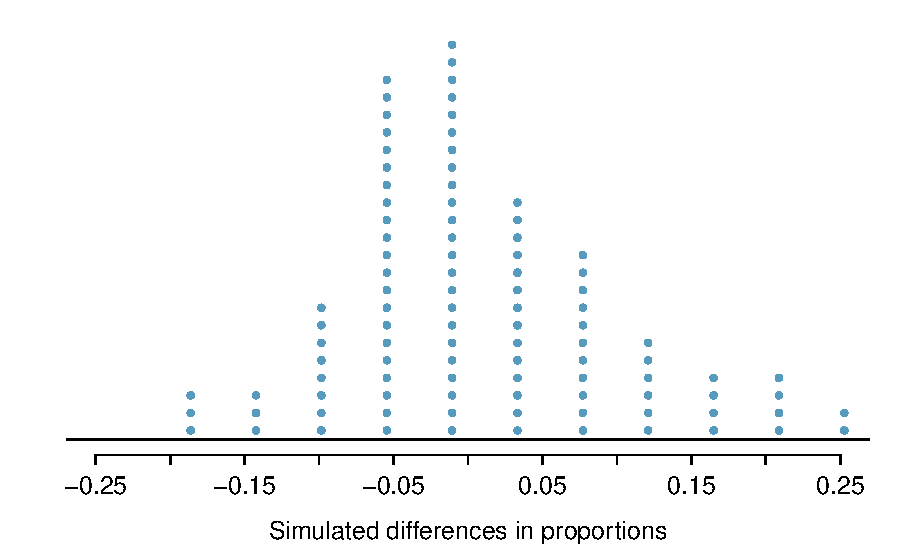
\includegraphics[width = 0.78\textwidth]{01/figures/eoce/heartTr/heartTr_RandHist} \\
\end{center}
}{}

\textA{\pagebreak}


%_________________
\subsection{Randomization case study: opportunity cost} % (Sections~\ref{caseStudyGenderDiscrimination}~\&~\ref{caseStudyOpportunityCost})}

% 3
\eoce{\qt{Side effects of Avandia, Part II} \label{AvandiaTrueFalseP2} Exercise~\ref{AvandiaTrueFalse} introduces a study that compares the rates of serious cardiovascular problems for diabetic patients on rosiglitazone and pioglitazone treatments. The table below summarizes the results of the study.
\begin{center}
\begin{tabular}{ll  cc c} 
								&				& \multicolumn{2}{c}{\textit{Cardiovascular problems}} \\
\cline{3-4}	
								&				& Yes 	& No 		& Total	\\
\cline{2-5}
\multirow{2}{*}{\textit{Treatment}}		& Rosiglitazone 	& 2,593	& 65,000		& 67,593 	\\
								& Pioglitazone		& 5,386 	& 154,592 	& 159,978\\
\cline{2-5}
								&Total			& 7,979	& 219,592		& 227,571
\end{tabular}
\end{center}
\begin{parts}
\item What proportion of all patients had cardiovascular problems?
\item If the type of treatment and having cardiovascular problems were independent (null hypothesis), about how many patients in the rosiglitazone group would we expect to have had cardiovascular problems?
\item We can investigate the relationship between outcome and treatment in this study using a randomization technique.  While in reality we would carry out the simulations required for randomization using statistical software, suppose we actually simulate using index cards. In order to simulate from the null hypothesis, which states that the outcomes were independent of the treatment, we write whether or not each patient had a cardiovascular problem on cards, shuffled all the cards together, then deal them into two groups of size 67,593 and 159,978. We repeat this simulation 10,000 times and each time record the number of people in the rosiglitazone group who had cardiovascular problems. Below is a relative frequency histogram of these counts.
\begin{subparts}
\item What are the claims being tested?
\item Compared to the number calculated in part (b), which would provide more support for the alternative hypothesis,  \textit{more} or \textit{fewer} patients with cardiovascular problems in the rosiglitazone group?
\item What do the simulation results suggest about the relationship between taking rosiglitazone and having cardiovascular problems in diabetic patients?
\end{subparts}
\begin{center}
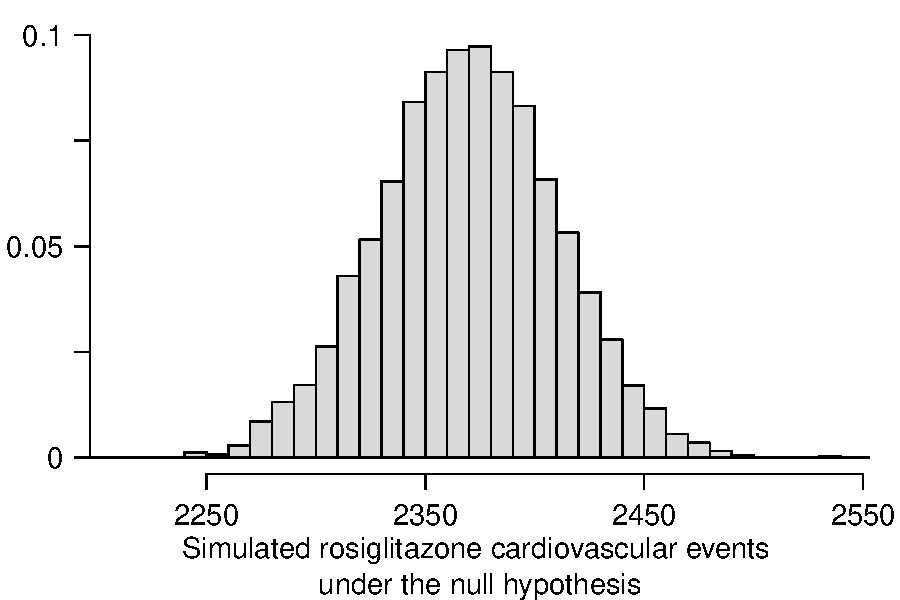
\includegraphics[width = 0.75\textwidth]{01/figures/eoce/avandia/avandia_RandHist} \\
\end{center}
\end{parts}
}{}

\textA{\pagebreak}


% 4
\eoce{\qt{Sinusitis and antibiotics, Part II} \label{sinusitisEOCEinCh2} Researchers studying the effect of antibiotic treatment compared to symptomatic treatment for acute sinusitis randomly assigned 166 adults diagnosed with sinusitis into two groups (as discussed in Exercise~\ref{sinusitis}). Participants in the antibiotic group received a 10-day course of an antibiotic, and the rest received symptomatic treatments as a placebo. These pills had the same taste and packaging as the antibiotic. At the end of the 10-day period patients were asked if they experienced improvement in symptoms since the beginning of the study. The distribution of responses is summarized below. \footfullcite{Garbutt:2012}
\begin{center}
\begin{tabular}{ll  cc c} 
			&				& \multicolumn{2}{c}{\textit{Self-reported}} \\
			&				& \multicolumn{2}{c}{\textit{improvement in symptoms}} \\
\cline{3-4}
			&							& Yes 	& No 	& Total	\\
\cline{2-5}
							&Antibiotic 	& 66	 	& 19		& 85 	\\
\raisebox{1.5ex}[0pt]{\textit{Treatment}}	& Placebo		& 65	 	& 16 	 	& 81 \\
\cline{2-5}
							&Total		& 131	& 35		& 166
\end{tabular}
\end{center}
\begin{parts}
\item What type of a study is this?
\item Does this study make use of blinding?
\item Compute the difference in the proportions of patients who self-reported an improvement in symptoms in the two groups: $\hat{p}_{antibiotic} - \hat{p}_{placebo}$.
\item At first glance, does antibiotic or placebo appear to be more effective for the treatment of sinusitis? Explain your reasoning using appropriate statistics.
\item There are two competing claims that this study is used to compare: the null hypothesis that the antibiotic has no impact and the alternative hypothesis that it has an impact. Write out these competing claims in easy-to-understand language and in the context of the application.
\item Below is a histogram of simulation results computed under the null hypothesis. In each simulation, the summary value reported was the number of patients who received antibiotics and self-reported an improvement in symptoms. Write a conclusion for the hypothesis test in plain language. (Hint: Does the value observed in the study, 66, seem unusual in this distribution generated under the null hypothesis?)
\begin{center}
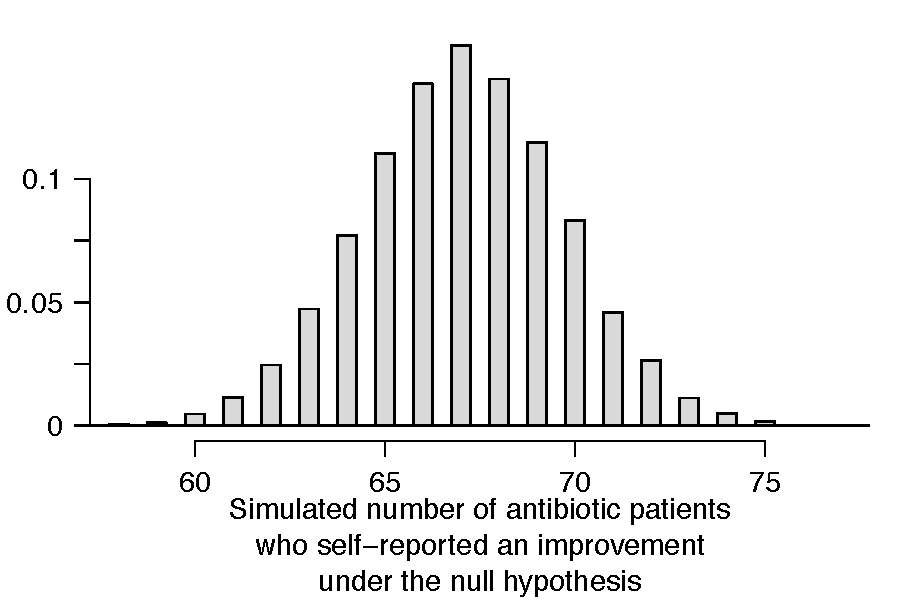
\includegraphics[width = 0.75\textwidth]{02/figures/eoce/sinusitis/sinusitis}
\end{center}
\end{parts}
}{}

\textA{\newpage}


%_________________
\subsection{Hypothesis testing}

% 5

\eoce{\qt{Social experiment, Part I} \label{socExpP1} A ``social experiment" conducted by a TV program questioned what people do when they see a very obviously bruised woman getting picked on by her boyfriend. On two different occasions at the same restaurant, the same couple was depicted. In one scenario the woman was dressed ``provocatively'' and in the other scenario the woman was dressed ``conservatively''. The table below shows how many restaurant diners were present under each scenario, and whether or not they intervened.
\begin{center}
\begin{tabular}{ll cc c} 
			&				& \multicolumn{2}{c}{\textit{Scenario}} \\
\cline{3-4}
							&			& Provocative	& Conservative 	& Total	\\
\cline{2-5}
\multirow{2}{*}{\textit{Intervene}}	&Yes 		& 5	 	& 15		& 20 	\\
							&No			& 15	 	& 10 	 	& 25 \\
\cline{2-5}
							&Total		& 20		& 25		& 45 \\
\end{tabular}
\end{center}
A simulation was conducted to test if people react differently under the two scenarios. 10,000 simulated differences were generated to construct the null distribution shown. The value $\hat{p}_{pr, sim}$ represents the proportion of diners who intervened in the simulation for the provocatively dressed woman, and $\hat{p}_{con, sim}$ is the proportion for the conservatively dressed woman.
\begin{center}
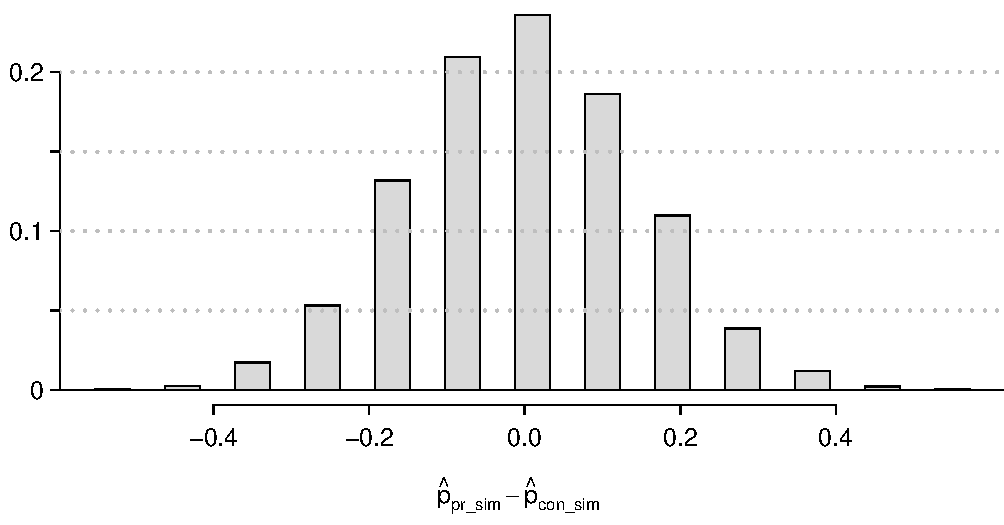
\includegraphics[width=0.9\textwidth]{03/figures/eoce/socExp/socExp}
\end{center}
\begin{parts}
\item What are the hypotheses? For the purposes of this exercise, you may assume that each observed person at the restaurant behaved independently, though we would want to evaluate this assumption more rigorously if we were reporting these results.
\item Calculate the observed difference between the rates of intervention under the provocative and conservative scenarios: $\hat{p}_{pr} - \hat{p}_{con}$.
\item Estimate the p-value using the figure above and determine the conclusion of the hypothesis test.
\end{parts}
}{}

\textA{\newpage}


% 6

\eoce{\qt{Is yawning contagious, Part I} \label{yawningContageousP1} An experiment conducted by the \textit{MythBusters}, a science entertainment TV program on the Discovery Channel, tested if a person can be subconsciously influenced into yawning if another person near them yawns. 50 people were randomly assigned to two groups: 34 to a group where a person near them yawned (treatment) and 16 to a group where there wasn't a person yawning near them (control). The following table shows the results of this experiment. \footfullcite{data:yawn}
\begin{center}
\begin{tabular}{ll cc c} 
			&				& \multicolumn{2}{c}{\textit{Group}} \\
\cline{3-4}
							&			& Treatment	& Control 	& Total	\\
\cline{2-5}
\multirow{2}{*}{\textit{Result}}		&Yawn 		& 10	 	& 4		& 14 	\\
							&Not Yawn	& 24	 	& 12 	 	& 36 \\
\cline{2-5}
							&Total		& 34		& 16		& 50 \\
\end{tabular}
\end{center}
A simulation was conducted to understand the distribution of the test statistic under the assumption of independence: having someone yawn near another person has no influence on if the other person will yawn. In order to conduct the simulation, a researcher wrote yawn on 14 index cards and not yawn on 36 index cards to indicate whether or not a person yawned. Then he shuffled the cards and dealt them into two groups of size 34 and 16 for treatment and control, respectively. He counted how many participants in each simulated group yawned in an apparent response to a nearby yawning person, and calculated the difference between the simulated proportions of yawning as $\hat{p}_{trtmt,sim} - \hat{p}_{ctrl,sim}$. This simulation was repeated 10,000 times using software to obtain 10,000 differences that are due to chance alone. The histogram shows the distribution of the simulated differences.
\begin{center}
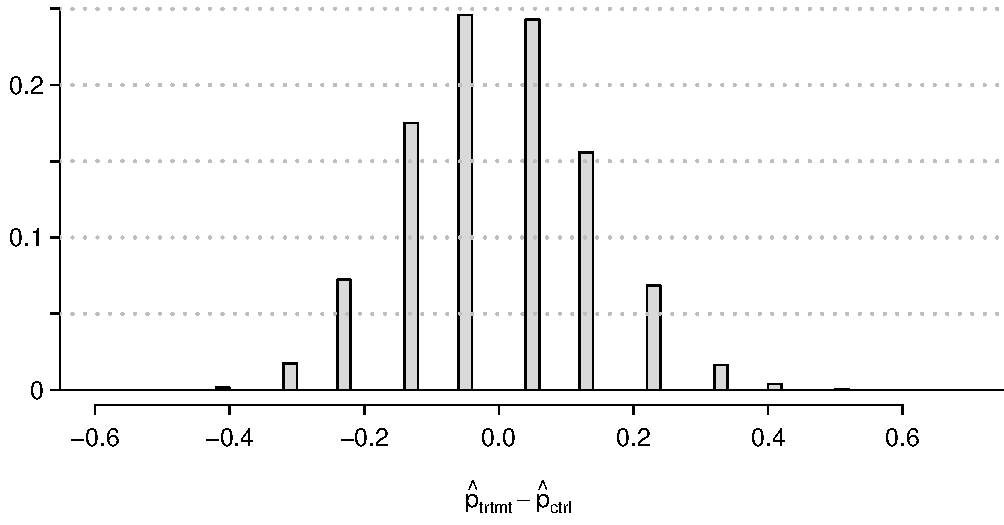
\includegraphics[width=0.9\textwidth]{03/figures/eoce/yawn/yawn}
\end{center}

\begin{parts}
\item What are the hypotheses?
\item Calculate the observed difference between the yawning rates under the two scenarios.
\item Estimate the p-value using the figure above and determine the conclusion of the hypothesis test.
\end{parts}
}{}

\textA{\pagebreak}

% 7

\eoce{\qt{Social experiment, Part II} In Exercise~\ref{socExpP1}, we encountered a scenario where researchers were evaluating the impact of the way someone is dressed against the actions of people around them. In that exercise, researchers may have believed that dressing provocatively may reduce the chance of bystander intervention. One might be tempted to use a one-sided hypothesis test for this study. Discuss the drawbacks of doing so in 1-3 sentences.}{}

% 8

\eoce{\qt{Is yawning contagious, Part II} Exercise~\ref{yawningContageousP1} describes an experiment by Myth Busters, where they examined whether a person yawning would affect whether others to yawn. The traditional belief is that yawning is contagious -- one yawn can lead to another yawn, which might lead to another, and so on. In that exercise, there was the option of selecting a one-sided or two-sided test. Which would you recommend (or which did you choose)? Justify your answer in 1-3 sentences.}{}


%_________________
\subsection{Simulation case studies} % (Section~\ref{SimulationCaseStudies})}

% 1

%\eoce{\qt{Bullying in schools} A 2012 Survey USA poll asked Florida residents how big of a problem they thought bullying was in local schools. 9 out of 191 18-34 year olds responded that bullying is no problem at all. Using these data, is it appropriate to construct a confidence interval using the formula $\hat{p} \pm z^\star \sqrt{ \hat{p}(1-\hat{p})/n }$ for the true proportion of 18-34 year old Floridians who think bullying is no problem at all? If it is appropriate, construct the confidence interval. If it is not, explain why.
%}{}

% 2

%\eoce{\qt{Choose a test} We would like to test the following hypotheses:
%\begin{hyp}
%\item[] $H_0: p = 0.1$
%\item[] $H_A: p \ne 0.1$
%\end{hyp}
%The sample size is 120 and the sample proportion is 8.5\%. Determine which of the below test(s) is/are appropriate for this situation and explain your reasoning.
%\begin{multicols}{2}
%\begin{romanparts}
%\item Z test for a proportion\index{Z test},\\
%	i.e. proportion test using normal model
%\item Z test for comparing two proportions
%\item $\chi^2$ test of independence
%\item Simulation test for a proportion
%\item $t$ test for a mean
%\item ANOVA
%\end{romanparts}
%\end{multicols}
%}{}

% 3

\eoce{\qt{The Egyptian Revolution} \label{EgyptianRevolutionEOCE} A popular uprising that started on January 25, 2011 in Egypt led to the 2011 Egyptian Revolution. Polls show that about 69\% of American adults followed the news about the political crisis and demonstrations in Egypt closely during the first couple weeks following the start of the uprising. Among a random sample of 30 high school students, it was found that only 17 of them followed the news about Egypt closely during this time. \footfullcite{data:egypt}

\begin{parts}

\item Write the hypotheses for testing if the proportion of high school students who followed the news about Egypt is different than the proportion of American adults who did.

\item Calculate the proportion of high schoolers in this sample who followed the news about Egypt closely during this time.

\item Describe how to perform a simulation and, once you had results, how to estimate the p-value.

\item Below is a histogram showing the distribution of $\hat{p}_{sim}$ in 10,000 simulations under the null hypothesis. Estimate the p-value using the plot and determine the conclusion of the hypothesis test.
\begin{center}
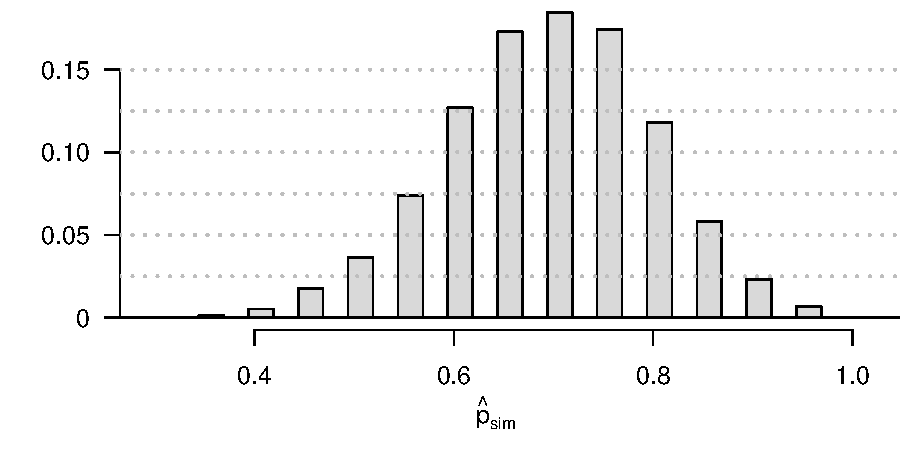
\includegraphics[width=0.65\textwidth]{03/figures/eoce/egypt/egypt}
\end{center}

\end{parts}
}{}

% 4

\eoce{\qt{Assisted Reproduction} \label{AssistedReproductionEOCE} Assisted Reproductive Technology (ART) is a collection of techniques that help facilitate pregnancy (e.g. in vitro fertilization). A 2008 report by the Centers for Disease Control and Prevention estimated that ART has been successful in leading to a live birth in 31\% of cases \footfullcite{web:art}. A new fertility clinic claims that their success rate is higher than average. A random sample of 30 of their patients yielded a success rate of 40\%. A consumer watchdog group would like to determine if this provides strong evidence to support the company's claim.
\begin{parts}
\item Write the hypotheses to test if the success rate for ART at this clinic is significantly higher than the success rate reported by the CDC.
\item Describe a setup for a simulation that would be appropriate in this situation and how the p-value can be calculated using the simulation results.
\item Below is a histogram showing the distribution of $\hat{p}_{sim}$ in 10,000 simulations under the null hypothesis. Estimate the p-value using the plot and use it to evaluate the hypotheses.
\item After performing this analysis, the consumer group releases the following news headline: ``Infertility clinic falsely advertises better success rates". Comment on the appropriateness of this statement.
\begin{center}
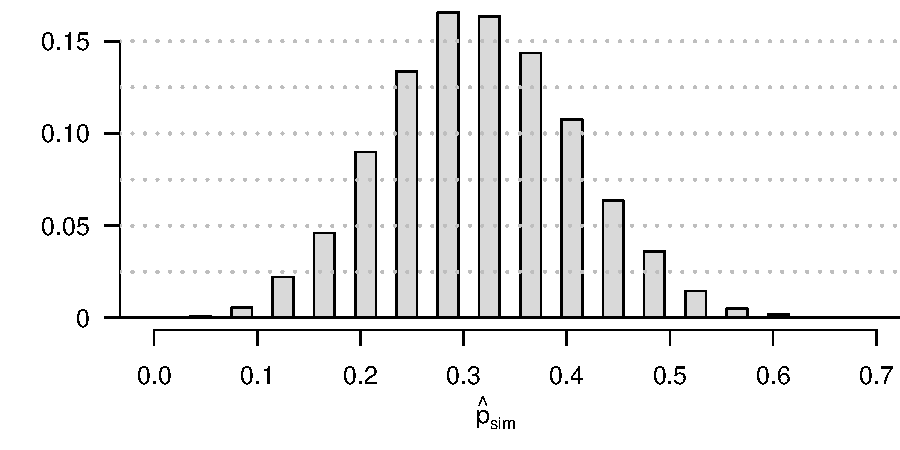
\includegraphics[width=0.7\textwidth]{03/figures/eoce/art/art}
\end{center}
\end{parts}
}{}

%_________________
\subsection{Central Limit Theorem} % (Section~\ref{})}

% 1 new

\eoce{\qt{Distribution of $\hat{p}$} Suppose the true population proportion were $p = 0.1$. The figure below shows what the distribution of a sample proportion looks like when the sample size is $n = 20$, $n = 100$, and $n = 500$. What does each point (observation) in each of the samples represent? Describe how the distribution of the sample proportion, $\hat{p}$, changes as $n$ becomes larger.
\begin{center}
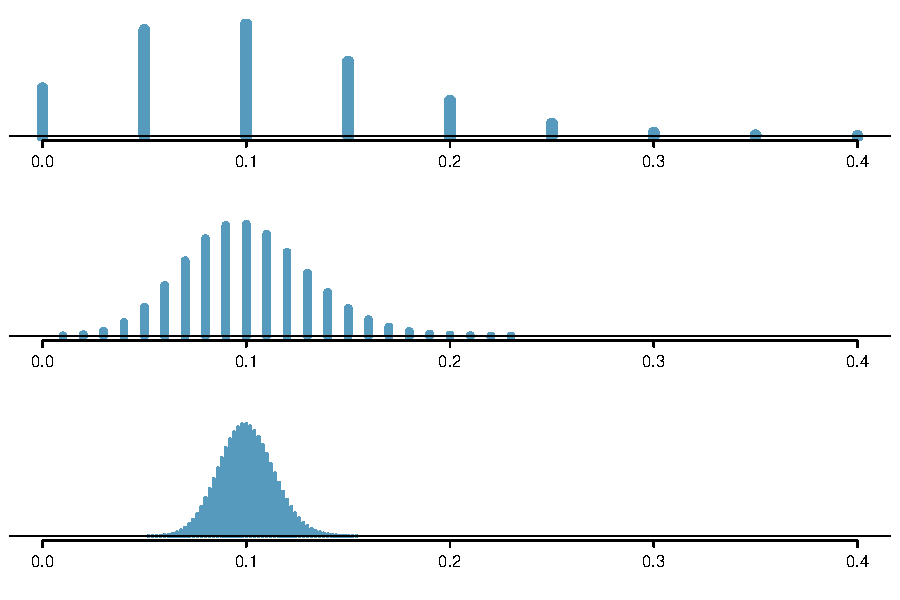
\includegraphics[width = 0.85\textwidth]{03/figures/eoce/eoce-p-hat-simulations/eoce-p-hat-simulations-p1}
\end{center}}{
%Each observation in each of the distributions represents the sample proportion ($\hat{p}$) from samples of size  $n = 20$, $n = 100$, and $n = 500$, respectively. The centers for all three distributions are at 0.10, the true population parameter. When $n$ is small, the distribution is skewed to the right and not smooth. As $n$ increases, the variability of the distribution (standard error) decreases, and the shape of the distribution becomes more unimodal and symmetric.
}

% 2 new

\textA{\newpage}

\eoce{\qt{Distribution of $\hat{p}$} Suppose the true population proportion were $p = 0.5$. The figure below shows what the distribution of a sample proportion looks like when the sample size is $n = 20$, $n = 100$, and $n = 500$. What does each point (observation) in each of the samples represent? Describe how the distribution of the sample proportion, $\hat{p}$, changes as $n$ becomes larger.
\begin{center}
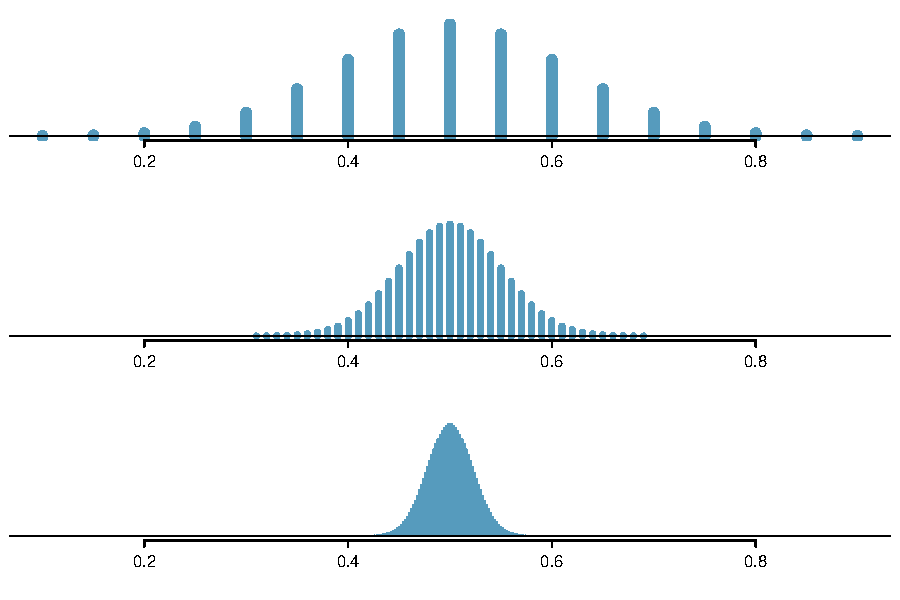
\includegraphics[width = 0.8\textwidth]{03/figures/eoce/eoce-p-hat-simulations/eoce-p-hat-simulations-p5}
\end{center}}{
%Each observation in each of the distributions represents the sample proportion ($\hat{p}$) from samples of size  $n = 20$, $n = 100$, and $n = 500$, respectively. Regardless of the sample size, the shapes of the distributions are symmetric, and centered at 0.50 the true population parameter. However as $n$ increases the variability of the distribution (standard error) decreases.
}

% 3 new 

\eoce{\qt{Distribution of $\hat{p}$} Suppose the true population proportion were $p = 0.95$. The figure below shows what the distribution of a sample proportion looks like when the sample size is $n = 20$, $n = 100$, and $n = 500$. What does each point (observation) in each of the samples represent? Describe how the distribution of the sample proportion, $\hat{p}$, changes as $n$ becomes larger.
\begin{center}
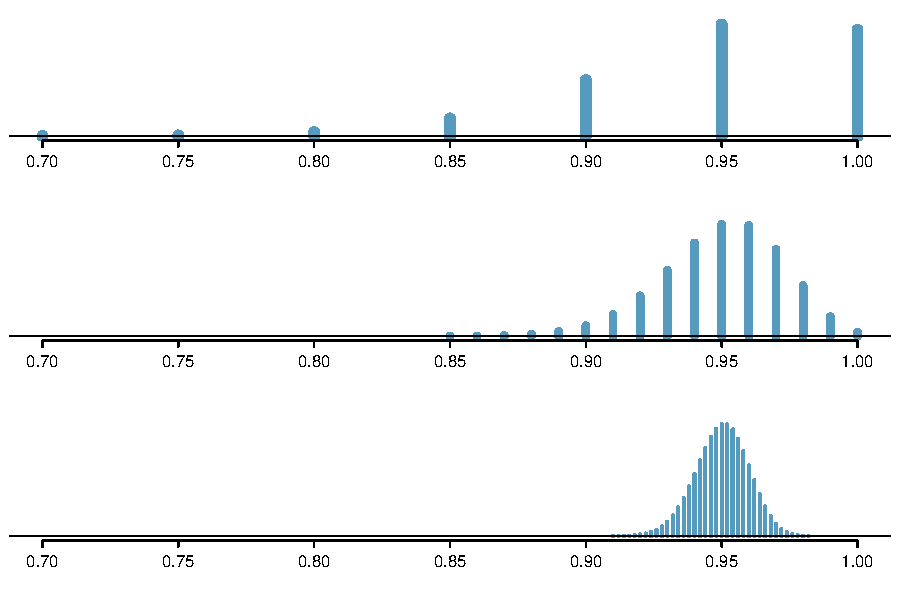
\includegraphics[width = 0.8\textwidth]{03/figures/eoce/eoce-p-hat-simulations/eoce-p-hat-simulations-p95}
\end{center}}{
%Each observation in each of the distributions represents the sample proportion ($\hat{p}$) from samples of size  $n = 20$, $n = 100$, and $n = 500$, respectively. The centers for all three distributions are at 0.95, the true population parameter. When $n$ is small, the distribution is skewed to the left and not smooth. As $n$ increases, the variability of the distribution (standard error) decreases, and the shape of the distribution becomes more unimodal and symmetric.
}

% 4 new 

\eoce{\qt{Re-examining the distributions of past exercises} Examine the distributions shown in Exercises~\ref{AvandiaTrueFalseP2}, \ref{sinusitisEOCEinCh2}, \ref{socExpP1}, \ref{yawningContageousP1}, \ref{EgyptianRevolutionEOCE}, and~\ref{AssistedReproductionEOCE}. Which distributions look symmetric and bell-shaped? Which appear to be overly ``discrete'' (not very smooth)?}{}


%_________________
\subsection{Normal distribution} % (Section~\ref{normDist})}

% 1

\eoce{\qt{Area under the curve, I} What percent of a standard normal distribution $N(\mu=0, \sigma=1)$ is found in each region? Be sure to draw a graph. \vspace{-3mm}
\begin{multicols}{4}
\begin{parts}
\item $Z < -1.35$
\item $Z > 1.48$
\item $-0.4 < Z < 1.5$
\item $|Z| > 2$
\end{parts}
\end{multicols}
}{}

% 2

\eoce{\qt{Area under the curve, II} What percent of a standard normal distribution $N(\mu=0, \sigma=1)$ is found in each region? Be sure to draw a graph. \vspace{-3mm}
\begin{multicols}{4}
\begin{parts}
\item $Z > -1.13$
\item $Z < 0.18$
\item $Z > 8$
\item $|Z| < 0.5$
\end{parts}
\end{multicols}
}{}

% 3

\eoce{\qt{Scores on the GRE, Part I\label{GRE}} A college senior who took the Graduate Record Examination exam scored 620 on the Verbal Reasoning section and 670 on the Quantitative Reasoning section. The mean score for Verbal Reasoning section was 462 with a standard deviation of 119, and the mean score for the Quantitative Reasoning was 584 with a standard deviation of 151. Suppose that both distributions are nearly normal.
\begin{parts}
\item Write down the short-hand for these two normal distributions.
\item What is her Z score on the Verbal Reasoning section? On the Quantitative Reasoning section? Draw a standard normal distribution curve and mark these two Z scores.
\item What do these Z scores tell you?
\item Relative to others, which section did she do better on?
\item Find her percentile scores for the two exams.
\item What percent of the test takers did better than her on the Verbal Reasoning section? On the Quantitative Reasoning section?
\item Explain why simply comparing her raw scores from the two sections would lead to the incorrect conclusion that she did better on the Quantitative Reasoning section.
\item If the distributions of the scores on these exams are not nearly normal, would your answers to parts (b) - (f) change? Explain your reasoning.
\end{parts}
}{}

% 4

\eoce{\qt{Triathlon times, Part I} \label{triathlon} In triathlons, it is common for racers to be placed into age and gender groups. Friends Leo and Mary both completed the Hermosa Beach Triathlon, where Leo competed in the \textit{Men, Ages 30 - 34} group while Mary competed in the \textit{Women, Ages 25 - 29} group. Leo completed the race in 1:22:28 (4948 seconds), while Mary completed the race in 1:31:53 (5513 seconds). Obviously Leo finished faster, but they are curious about how they did within their respective groups. Can you help them?
Here is some information on the performance of their groups:
\begin{itemize}
\setlength{\itemsep}{0mm}
\item The finishing times of the \textit{Men, Ages 30 - 34} group has a mean of 4313 seconds with a standard deviation of 583 seconds.
\item The finishing times of the \textit{Women, Ages 25 - 29} group has a mean of 5261 seconds with a standard deviation of 807 seconds.
\item The distributions of finishing times for both groups are approximately Normal.
\end{itemize}
Remember: a better performance corresponds to a faster finish.
\begin{parts}
\item Write down the short-hand for these two normal distributions.
\item What are the Z scores for Leo's and Mary's finishing times? What do these Z scores tell you?
\item Did Leo or Mary rank better in their respective groups? Explain your reasoning.
\item What percent of the triathletes did Leo finish faster than in his group?
\item What percent of the triathletes did Mary finish faster than in her group?
\item If the distributions of finishing times are not nearly normal, would your answers to parts (b) - (e) change? Explain your reasoning.
\end{parts}
}{}

% 5

\eoce{\qt{GRE scores, Part II} In Exercise~\ref{GRE} we saw two distributions for GRE scores: $N(\mu=462, \sigma=119)$ for the verbal part of the exam and $N(\mu=584, \sigma=151)$ for the quantitative part. Use this information to compute each of the following:
\begin{parts}
\item The score of a student who scored in the $80^{th}$ percentile on the Quantitative Reasoning section.
\item The score of a student who scored worse than 70\% of the test takers in the Verbal Reasoning section.
\end{parts}
}{}

% 6

\eoce{\qt{Triathlon times, Part II} In Exercise~\ref{triathlon} we saw two distributions for triathlon times: $N(\mu=4313, \sigma=583)$ for \emph{Men, Ages 30 - 34} and $N(\mu=5261, \sigma=807)$ for the \emph{Women, Ages 25 - 29} group. Times are listed in seconds. Use this information to compute each of the following:
\begin{parts}
\item The cutoff time for the fastest 5\% of athletes in the men's group, i.e. those who took the shortest 5\% of time to finish. 
\item The cutoff time for the slowest 10\% of athletes in the women's group. 
\end{parts}
}{}

% 7

\eoce{\qt{Temperatures in LA, Part I} \label{tempLA} The average daily high temperature in June in LA is 77\degree F with a standard deviation of 5\degree F. Suppose that the temperatures in June closely follow a normal distribution. 
\begin{parts}
\item What is the probability of observing an 83\degree F temperature or higher in LA during a randomly chosen day in June?
\item How cold are the coldest 10\% of the days during June in LA?
\end{parts}
}{}

% 8

\eoce{\qt{Portfolio returns} The Capital Asset Pricing Model is a financial model that assumes returns on a portfolio are normally distributed. Suppose a portfolio has an average annual return of 14.7\% (i.e. an average gain of 14.7\%) with a standard deviation of 33\%. A return of 0\% means the value of the portfolio doesn't change, a negative return means that the portfolio loses money, and a positive return means that the portfolio gains money.
\begin{parts}
\item What percent of years does this portfolio lose money, i.e. have a return less than 0\%?
\item What is the cutoff for the highest 15\% of annual returns with this portfolio?
\end{parts}
}{}

% 9

\eoce{\qt{Temperatures in LA, Part II} Exercise~\ref{tempLA} states that average daily high temperature in June in LA is 77\degree F with a standard deviation of 5\degree F, and it can be assumed that they to follow a normal distribution. We use the following equation to convert \degree F (Fahrenheit) to \degree C (Celsius):
\[ C = (F - 32) \times \frac{5}{9}. \]
\begin{parts}
\item Write the probability model for the distribution of temperature in \degree C in June in LA.
\item What is the probability of observing a 28\degree C (which roughly corresponds to 83\degree F) temperature or higher in June in LA? Calculate using the \degree C model from part (a).
\item Did you get the same answer or different answers in part (b) of this question and part (a) of Exercise~\ref{tempLA}? Are you surprised? Explain.
\end{parts}
}{}

% 10

\eoce{\qt{Heights of 10 year olds} Heights of 10 year olds, regardless of gender, closely follow a normal distribution with mean 55 inches and standard deviation 6 inches.
\begin{parts}
\item What is the probability that a randomly chosen 10 year old is shorter than 48 inches?
\item What is the probability that a randomly chosen 10 year old is between 60 and 65 inches?
\item If the tallest 10\% of the class is considered ``very tall", what is the height cutoff for ``very tall"?
\item The height requirement for \textit{Batman the Ride} at Six Flags Magic Mountain is 54 inches. What percent of 10 year olds cannot go on this ride?
\end{parts}
}{}

% 11
\textA{\pagebreak}

\eoce{\qt{Auto insurance premiums} Suppose a newspaper article states that the distribution of auto insurance premiums for residents of California is approximately normal with a mean of \$1,650. The article also states that 25\% of California residents pay more than \$1,800. 
\begin{parts}
\item What is the Z score that corresponds to the top 25\% (or the $75^{th}$ percentile) of the standard normal distribution?
\item What is the mean insurance cost? What is the cutoff for the 75th percentile?
\item Identify the standard deviation of insurance premiums in LA.
\end{parts}
}{}

% 12

\eoce{\qt{Speeding on the I-5, Part I} \label{i5} The distribution of passenger vehicle speeds traveling on the Interstate 5 Freeway (I-5) in California is nearly normal with a mean of 72.6 miles/hour and a standard deviation of 4.78 miles/hour.\footfullcite{Johnson+Murray:2010}
\begin{parts}
\item What percent of passenger vehicles travel slower than 80 miles/hour?
\item What percent of passenger vehicles travel between 60 and 80 miles/hour?
\item How fast do the fastest 5\% of passenger vehicles travel?
\item The speed limit on this stretch of the I-5 is 70 miles/hour. Approximate what percentage of the passenger vehicles travel above the speed limit on this stretch of the I-5.
\end{parts}
}{}

% 13

\eoce{\qt{Overweight baggage} Suppose weights of the checked baggage of airline passengers follow a nearly normal distribution with mean 45 pounds and standard deviation 3.2 pounds. Most airlines charge a fee for baggage that weigh in excess of 50 pounds. Determine what percent of airline passengers incur this fee.
}{}

% 14

\eoce{\qt{Find the SD} Find the standard deviation of the distribution in the following situations.
\begin{parts}
\item  MENSA is an organization whose members have IQs in the top 2\% of the population. IQs are normally distributed with mean 100, and the minimum IQ score required for admission to MENSA is 132.
\item Cholesterol levels for women aged 20 to 34 follow an approximately normal distribution with mean 185 milligrams per deciliter (mg/dl). Women with cholesterol levels above 220 mg/dl are considered to have high cholesterol and about 18.5\% of women fall into this category.
\end{parts}
}{}

% 15

\eoce{\qt{Buying books on Ebay} The textbook you need to buy for your chemistry class is expensive at the college bookstore, so you consider buying it on Ebay instead. A look at past auctions suggest that the prices of that chemistry textbook have an approximately normal distribution with mean \$89 and standard deviation \$15. 
\begin{parts}

\item What is the probability that a randomly selected auction for this book closes at more than \$100?

\item Ebay allows you to set your maximum bid price so that if someone outbids you on an auction you can automatically outbid them, up to the maximum bid price you set. If you are only bidding on one auction, what are the advantages and disadvantages of setting a bid price too high or too low? What if you are bidding on multiple auctions?

\item If you watched 10 auctions, roughly what percentile might you use for a maximum bid cutoff to be somewhat sure that you will win one of these ten auctions? Is it possible to find a cutoff point that will ensure that you win an auction?

\item If you are willing to track up to ten auctions closely, about what price might you use as your maximum bid price if you want to be somewhat sure that you will buy one of these ten books?

\end{parts}
}{}

% 16
\textA{\pagebreak}

\eoce{\qt{SAT scores} SAT scores (out of 2400) are distributed normally with a mean of 1500 and a standard deviation of 300. Suppose a school council awards a certificate of excellence to all students who score at least 1900 on the SAT, and suppose we pick one of the recognized students at random. What is the probability this student's score will be at least 2100? (The material covered in Section~\ref{conditionalProbabilitySection} would be useful for this question.)
}{}

% 17

\eoce{\qt{Scores on stats final, Part I} \label{statsScores} Below are final exam scores of 20 Introductory Statistics students. 
\[ \stackrel{1}{57}, \stackrel{2}{66}, \stackrel{3}{69}, \stackrel{4}{71}, \stackrel{5}{72}, \stackrel{6}{73}, \stackrel{7}{74}, \stackrel{8}{77}, \stackrel{9}{78}, \stackrel{10}{78}, \stackrel{11}{79}, \stackrel{12}{79}, \stackrel{13}{81}, \stackrel{14}{81}, \stackrel{15}{82}, \stackrel{16}{83}, \stackrel{17}{83}, \stackrel{18}{88}, \stackrel{19}{89}, \stackrel{20}{94} \]
The mean score is 77.7 points. with a standard deviation of 8.44 points. Use this information to determine if the scores approximately follow the 68-95-99.7\% Rule.
}{}

% 18

\eoce{\qt{Heights of female college students, Part I} \label{collegeFemHeights} Below are heights of 25 female college students.
\[ \stackrel{1}{54}, \stackrel{2}{55}, \stackrel{3}{56}, \stackrel{4}{56}, \stackrel{5}{57}, \stackrel{6}{58}, \stackrel{7}{58}, \stackrel{8}{59}, \stackrel{9}{60}, \stackrel{10}{60}, \stackrel{11}{60}, \stackrel{12}{61}, \stackrel{13}{61}, \stackrel{14}{62}, \stackrel{15}{62}, \stackrel{16}{63}, \stackrel{17}{63}, \stackrel{18}{63}, \stackrel{19}{64}, \stackrel{20}{65}, \stackrel{21}{65}, \stackrel{22}{67}, \stackrel{23}{67}, \stackrel{24}{69}, \stackrel{25}{73} \]
The mean height is 61.52 inches with a standard deviation of 4.58 inches. Use this information to determine if the heights approximately follow the 68-95-99.7\% Rule.
}{}

% 19

\eoce{\qt{Scores on stats final, Part II} Exercise~\ref{statsScores} lists the final exam scores of 20 Introductory Statistics students. Do these data appear to follow a normal distribution? Explain your reasoning using the graphs provided below.
\begin{center}
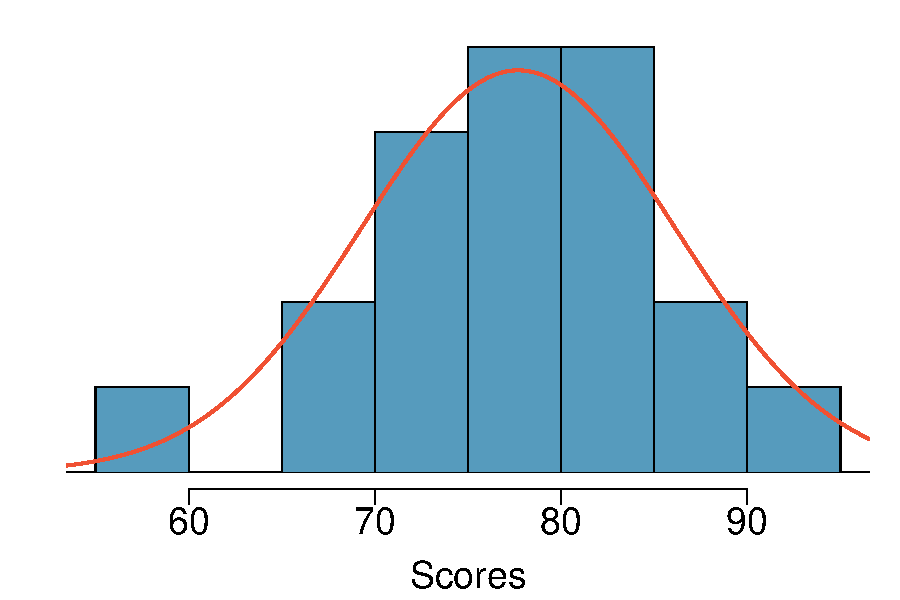
\includegraphics[width=0.46\textwidth]{02/figures/eoce/scores/scores_hist}\ \ \ \ 
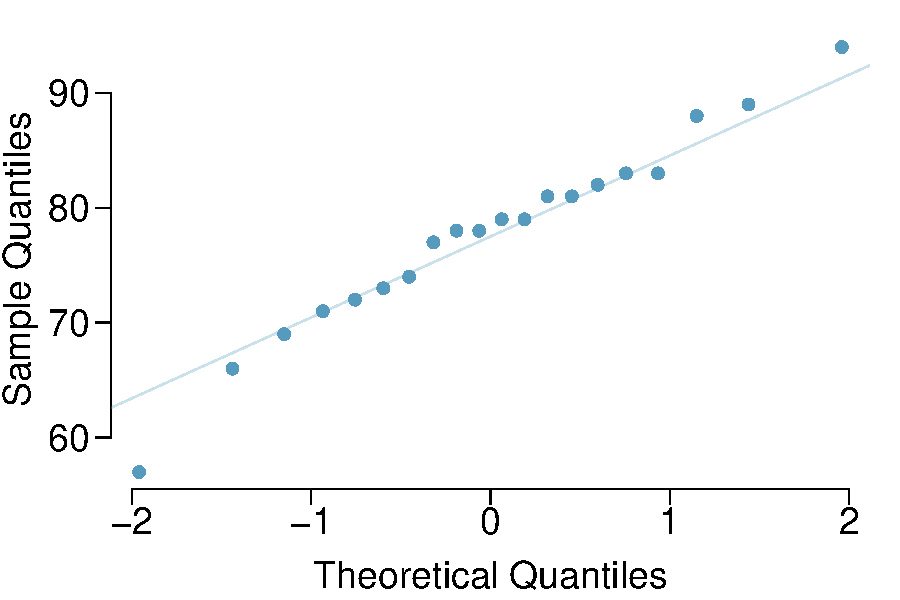
\includegraphics[width= 0.46\textwidth]{02/figures/eoce/scores/scores_qq}
\end{center}
}{}

% 20

\eoce{\qt{Heights of female college students, Part II} Exercise~\ref{collegeFemHeights} lists the heights of 25 female college students. Do these data appear to follow a normal distribution? Explain your reasoning using the graphs provided below.
\begin{center}
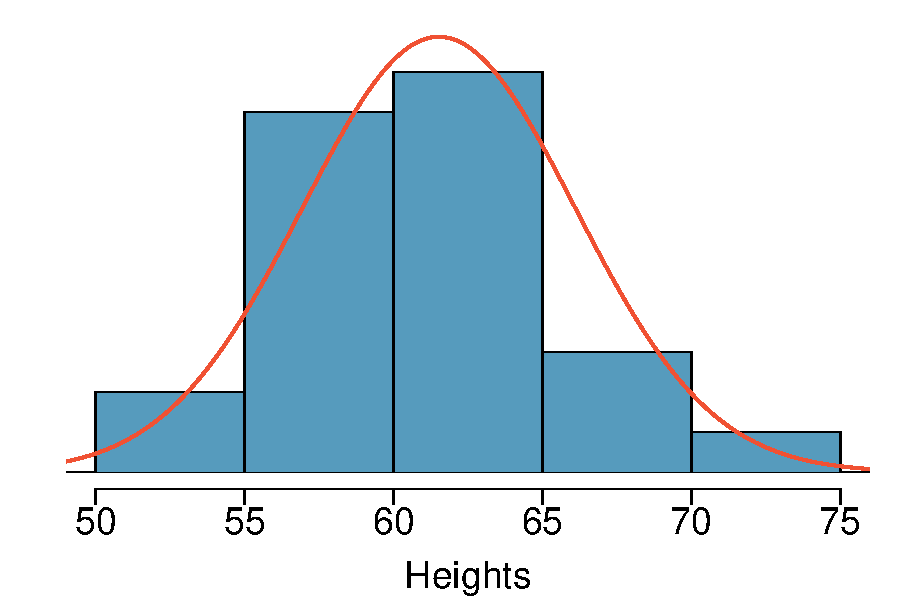
\includegraphics[width= 0.46\textwidth]{02/figures/eoce/heightsFcoll/heightsFcoll_hist}\ \ \ \ 
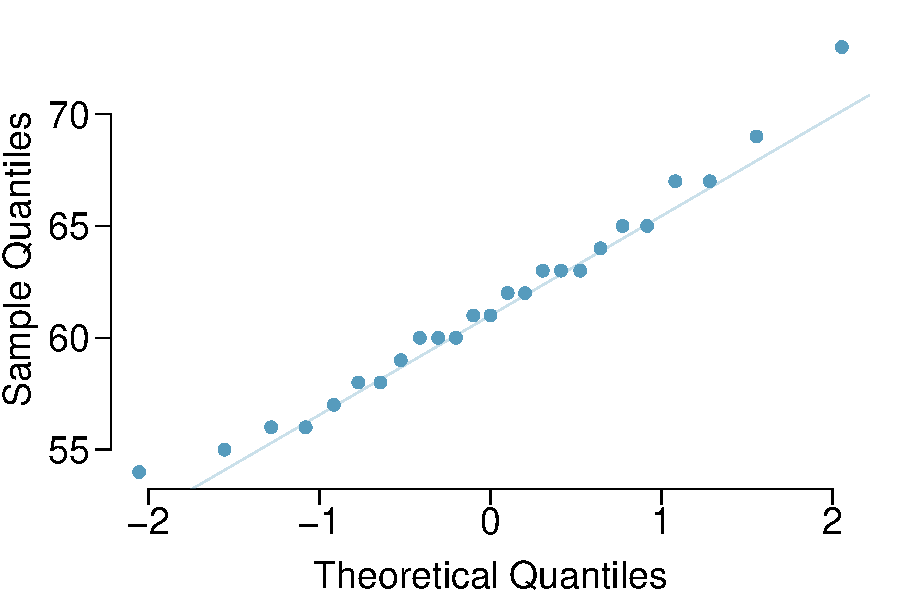
\includegraphics[width= 0.46\textwidth]{02/figures/eoce/heightsFcoll/heightsFcoll_qq}
\end{center}
}{}

\textPE{\pagebreak}

%_________________
\subsection{Applying the normal model} % (Section~\ref{ApplyingTheNormalModel})}

\eoce{\qt{Side effects of Avandia, Part III} \label{AvandiaTrueFalseP3}
Exercise~\ref{AvandiaTrueFalse} introduces a study that compares the rates of serious cardiovascular problems for diabetic patients on rosiglitazone and pioglitazone treatments. The table below summarizes the results of the study.
\begin{center}
\begin{tabular}{ll  cc c} 
								&				& \multicolumn{2}{c}{\textit{Cardiovascular problems}} \\
\cline{3-4}	
								&				& Yes 	& No 		& Total	\\
\cline{2-5}
\multirow{2}{*}{\textit{Treatment}}		& Rosiglitazone 	& 2,593	& 65,000		& 67,593 	\\
								& Pioglitazone		& 5,386 	& 154,592 	& 159,978\\
\cline{2-5}
								&Total			& 7,979	& 219,592		& 227,571
\end{tabular}
\end{center}
\begin{parts}
\item Write a set of hypotheses comparing the rates for cardiovascular problems for the two treatments. %Write a set of hypotheses appropriate for the context.
\item Compute the observed difference in rates for cardiovascular problems in the two treatments.
\item This study is a suitable candidate for applying a normal distribution. If there really was no difference in the rates of cardiovascular problems and the two drugs under consideration, we can use a normal model with mean 0 and standard error 0.00084. Using this model, compute an appropriate p-value.
\item Write a suitable conclusion based on your p-value. Use a significance level of $\alpha = 0.01$.
\end{parts}}{}

\eoce{\qt{Crime concerns in China} A~2013 poll found that 24\% of Chinese adults see crime as a very big problem, and the standard error for this estimate, which can reasonably be modeled using a normal distribution, is $SE = 1.8\%$.\footnote{\href{http://www.pewglobal.org/2013/09/19/environmental-concerns-on-the-rise-in-china}{Environmental Concerns on the Rise in China}. September 19, 2013. Pew Research.} Suppose an issue will get special attention from the Chinese government if more than 1-in-5 Chinese adults express concern on an issue.
\begin{parts}
\item Construct hypotheses regarding whether or not crime should receive special attention by the Chinese government according to the 1-in-5 guideline.
\item Discuss the appropriateness of using a one-sided or two-sided test for this exercise. \emph{Consider:} for this decision process, would we care about one or both directions?
\item Should crime receive special attention? Use a hypothesis test to justify your answer.
\end{parts}}{}


%_________________
\subsection{Confidence intervals} % (Section~\ref{})}

% 1

\eoce{\qt{Chronic illness, Part I} \label{ChronicIllnessP1}
In 2013, the Pew Research Foundation reported that ``45\% of U.S. adults report that they live with one or more chronic conditions''.\footnote{\href{http://pewinternet.org/Reports/2013/The-Diagnosis-Difference.aspx}{The Diagnosis Difference}. November 26, 2013. Pew Research.} However, this value was based on a sample, so it may not be a perfect estimate for the population parameter of interest on its own. The study reported a standard error of about 1.2\%, and a normal model may reasonably be used in this setting. Create a 95\% confidence interval for the proportion of U.S. adults who live with one or more chronic conditions. Also interpret the confidence interval in the context of the study.}
{
%$0.45 \pm 1.96 \times 0.012 = (0.426, 0.474)$ \\
%We are 95\% confident that 42.6\% to 47.4\% of U.S. adults live with one or more chronic conditions.
}

% 2

\eoce{\qt{Twitter users and news, Part I} A poll conducted in 2013 found that 52\% of U.S. adult Twitter users get at least some news on Twitter.\footnote{\href{http://www.journalism.org/2013/11/04/twitter-news-consumers-young-mobile-and-educated}{Twitter News Consumers: Young, Mobile and Educated}. November 4, 2013. Pew Research.} The standard error for this estimate was 2.4\%, and a normal distribution may be used to model the sample proportion. Construct a 99\% confidence interval for the fraction of U.S. adult Twitter users who get some news on Twitter, and interpret the confidence interval in context.}{}

\textA{\pagebreak}

% 3

\eoce{\qt{Chronic illness, Part II} In 2013, the Pew Research Foundation reported that ``45\% of U.S. adults report that they live with one or more chronic conditions'', and the standard error for this estimate is 1.2\%.
Identify each of the following statements as true or false. Provide an explanation to justify each of your answers.
\begin{parts}
\item We can say with certainty that the confidence interval from Exerise~\ref{ChronicIllnessP1} contains the true percentage of U.S. adults who suffer from a chronic illness.
\item If we repeated this study 1,000 times and constructed a 95\% confidence interval for each study, then approximately 950 of those confidence intervals would contain the true fraction of U.S. adults who suffer from chronic illnesses.
\item The poll provides statistically significant evidence (at the $\alpha = 0.05$ level) that the percentage of U.S. adults who suffer from chronic illnesses is below 50\%.
\item Since the standard error is 1.2\%, only 1.2\% of people in the study communicated uncertainty about their answer.
\end{parts}}
{
%\begin{parts}
%\item False, we're only 95\% confident.
%\item True, this is the definition of the confidence level.
%\item True, the equivalent significance level of a one sided hypothesis test for a 95\% confidence interval is indeed 2.5\%, and since the interval lies below 50\% this statement is correct. % would need revision of this part
%\item False, the 1.2\% measures the uncertainty associated with the sample proportion (the point estimate) not the uncertainty of individual observations, uncertainty in the sense of not being sure of one's answer to a survey question.
%\end{parts}
}

% 4

\eoce{\qt{Twitter users and news, Part II} A poll conducted in 2013 found that 52\% of U.S. adult Twitter users get at least some news on Twitter, and the standard error for this estimate was 2.4\%. Identify each of the following statements as true or false. Provide an explanation to justify each of your answers.
\begin{parts}
\item The data provide statistically significant evidence that more than half of U.S. adult Twitter users get some news through Twitter. Use a significance level of $\alpha = 0.01$.
\item Since the standard error is 2.4\%, we can conclude that 97.6\% of all U.S. adult Twitter users were included in the study.
\item If we want to reduce the standard error of the estimate, we should collect less data.
\item If we construct a 90\% confidence interval for the percentage of U.S. adults Twitter users who get some news through Twitter, this confidence interval will be wider than a corresponding 99\% confidence interval.
\end{parts}}{}



